\documentclass{article}
\usepackage{graphicx} % new way of doing eps files
\usepackage{listings} % nice code layout
\usepackage[usenames]{color} % color
\definecolor{listinggray}{gray}{0.9}
\definecolor{graphgray}{gray}{0.7}
\definecolor{ans}{rgb}{1,0,0}
\definecolor{blue}{rgb}{0,0,1}
% \Verilog{title}{label}{file}
\newcommand{\Verilog}[3]{
  \lstset{language=Verilog}
  \lstset{backgroundcolor=\color{listinggray},rulecolor=\color{blue}}
  \lstset{linewidth=\textwidth}
  \lstset{commentstyle=\textit, stringstyle=\upshape,showspaces=false}
  \lstset{frame=tb}
  \lstinputlisting[caption={#1},label={#2}]{#3}
}


\author{Cameron Anderson}
\title{Class Report 2: Block Memory}

\begin{document}
\maketitle

\section{Introduction}
The goal of this project is to use the seven-segment display and binary switches to read and write to and from the block memory within the Nexys 4 DDR prototyping board. For this project, the data and address registers are each 32 bits. The seven-segment display has 8 digits and can display the full range of hexidecimal digits at each of the 8 locations. With only 16 switches, the registers will need to be divided into MSB and LSB registers to read in the switches.

\section{Experimental Plan}
\begin{figure}
\begin{center}
\caption{State Machine for using Block Memory}\label{fig:blockmemstatemachine}
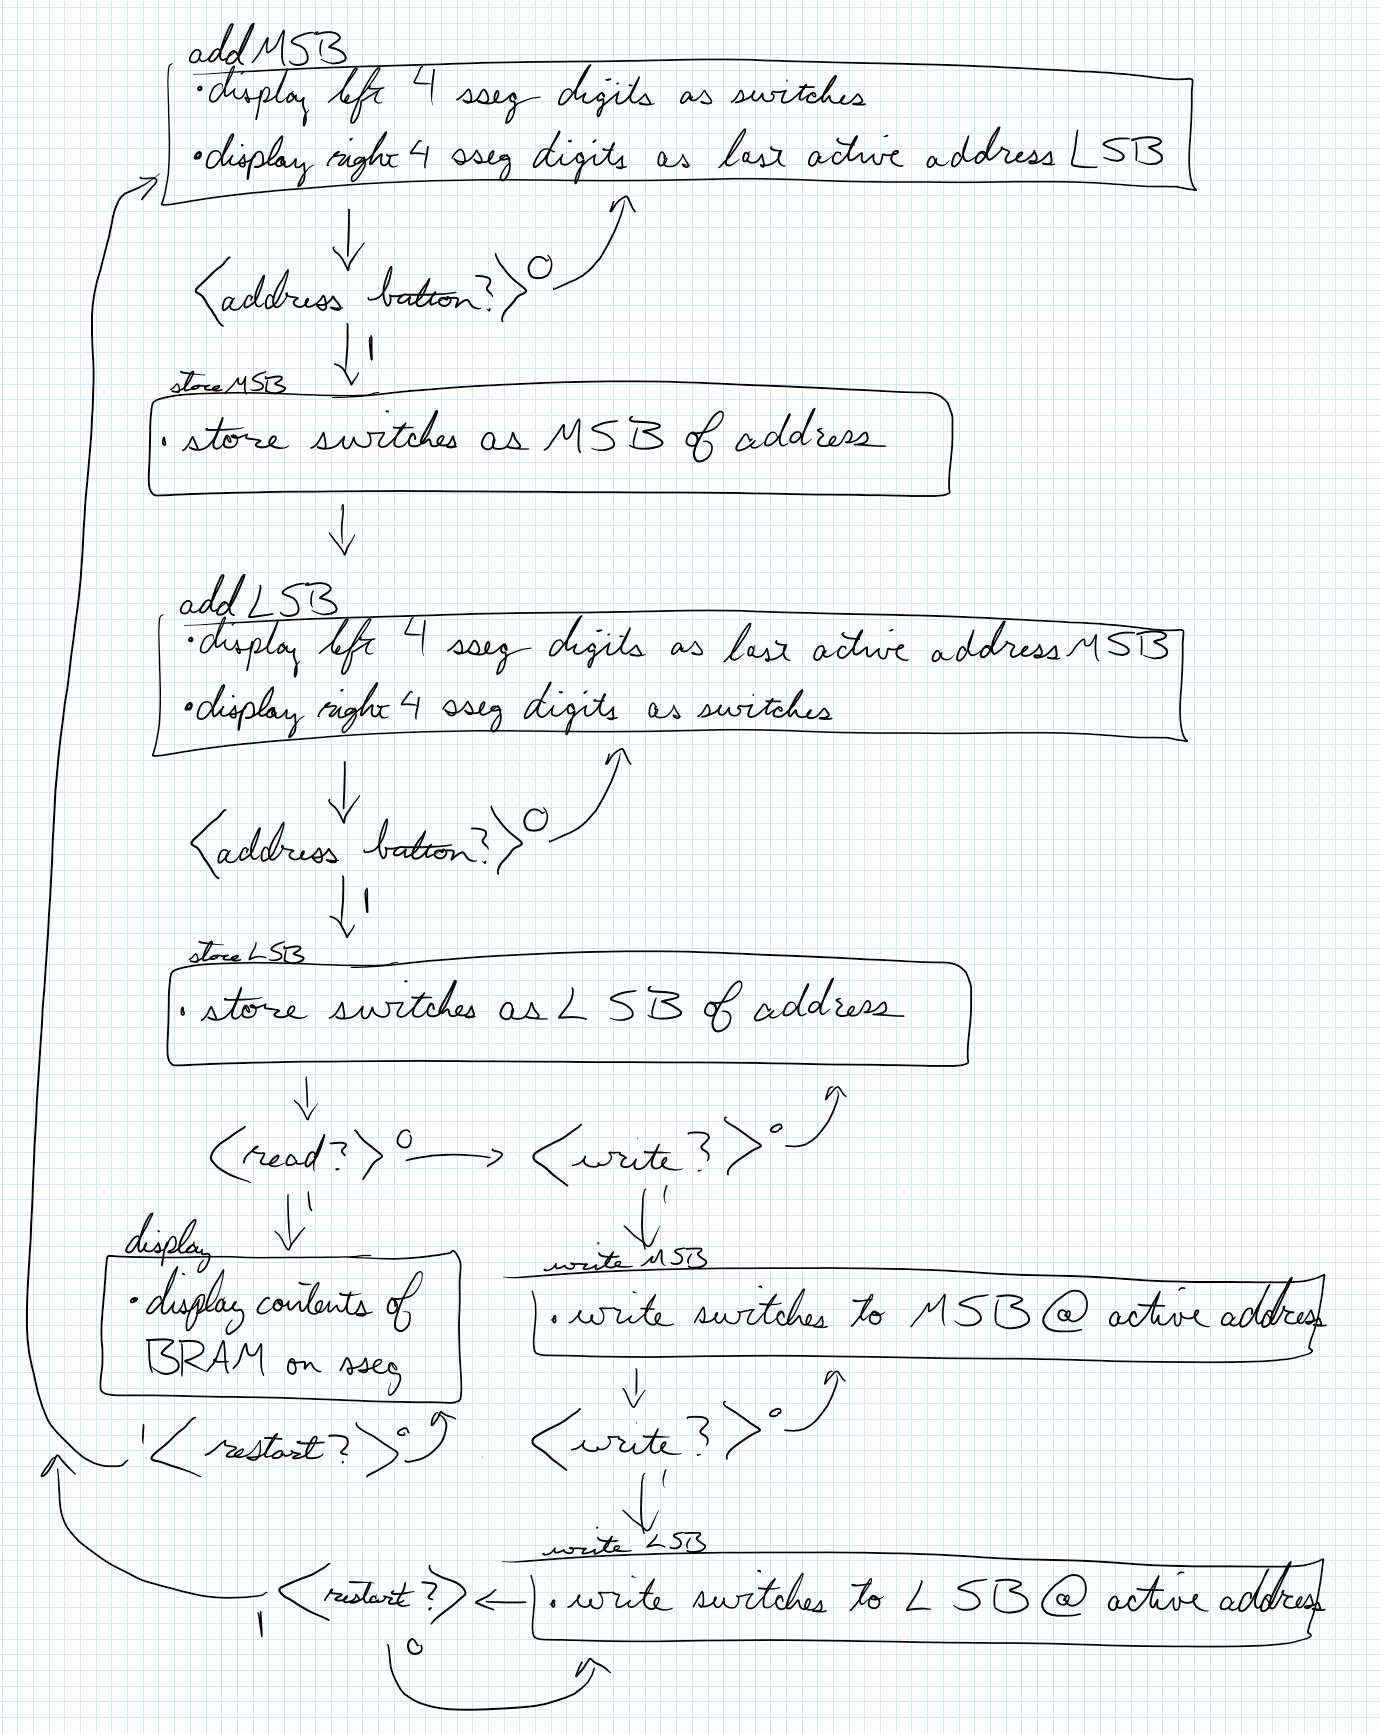
\includegraphics[width=0.9\textwidth]{blockmemstatemachine.jpg}
\end{center}
\end{figure}
     
\section{Analysis}
%
%
%\begin{figure}
%\begin{center}
%\caption{Timing diagram for the instruction memory test.}\label{fig:instrsim}
%\includegraphics[width=0.9\textwidth]{../images/instr_mem_sim.png}
%\end{center}
%\end{figure}
%
%\begin{figure}
%\begin{center}
%	\caption{Timing diagram for the iFetch module test.}\label{fig:ifetchsim}
%	\includegraphics[width=0.9\textwidth]{../images/iFetch_sim.png}
%\end{center}
%\end{figure}

\section{Conclusion}



\end{document} 